%!TeX root = ../main.tex

{\raggedright\large\textbf{Local feature compression using autoencoders - SfM tests}}\smallskip \\ 
Design a compression strategy for local SURF descriptors using autoencoders. Training data can be generated using the images of dataset Portello and Castle. Testing must be done on dataset FountainP-11 and Tiso (available at \url{https://github.com/openMVG/SfM_quality_evaluation/tree/master/Benchmarking_Camera_Calibration_2008} and \url{http://www.dei.unipd.it/~sim1mil/materiale/3Drecon/}). Software must be implemented in MATLAB, Keras or Pytorch. \\ \textbf{Testing on 3D reconstruction using SfM:} The reconstructed descriptors (only for the test set) are used to perform a SfM reconstruction using COLMAP (using the two test dataset). \\
Programming languages: MATLAB/Python/C++.

\section{Introduction}

\subsection{Descriptors in general}
In computer vision, visual descriptors or image descriptors are descriptions of the visual features of the contents in images, videos, or algorithms or applications that produce such descriptions. They describe elementary characteristics such as the shape, the color, the texture or the motion, among others\footnote{\url{https://en.wikipedia.org/wiki/Visual_descriptor}, 01/02/21}. A feature detector (\emph{extractor}) is an algorithm taking an image as input and outputting a set of regions (``local features'' = ``Interest Points'' = ``Keypoints'' = ``Feature Points''). A descriptor is computed on an image region defined by a detector. The descriptor is a representation of the image function (colour, shape, ...) in the region (typically an array). Two key operations are related to feature extraction:
\begin{itemize}
\item Feature detection: extract the features of interest
\item Feature description: associate a descriptor to each feature in order to distinguish from the others
\end{itemize}
There are many pre-defined descriptors available to the users. Some of them are reported in fig.\ref{fig:descriptors}.

\begin{figure}[h!]
    \centering
    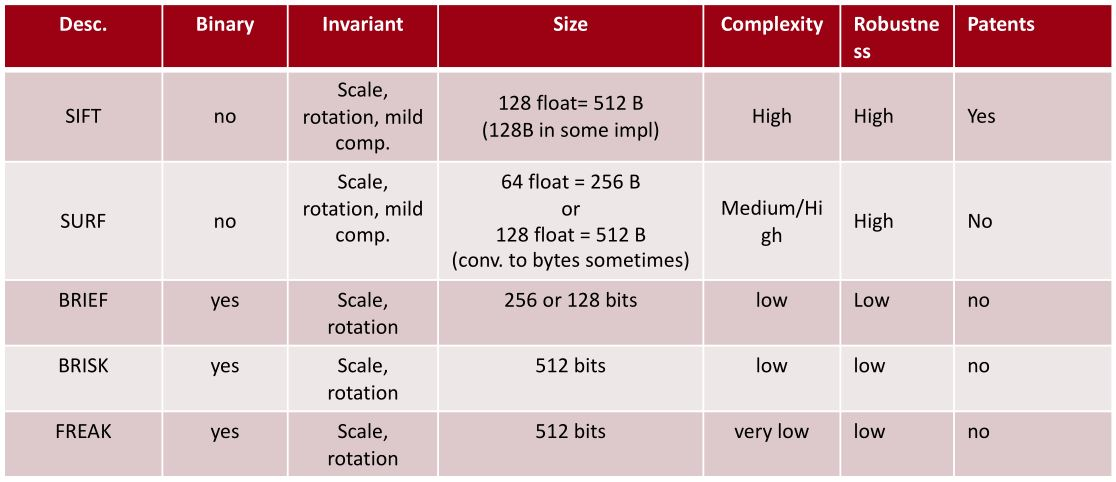
\includegraphics[width=0.9\textwidth]{images/Descriptors.jpg}
    \caption{Common algorithms for feature description.}
    \label{fig:descriptors}    
\end{figure}


\subsection{Speeded Up Robust Features (SURF)}
In computer vision, Speeded Up Robust Features (SURF) is a local feature detector and descriptor. It can be used for tasks such as object recognition, image registration, classification, or 3D reconstruction. It is partly inspired by the Scale-Invariant Feature Transform (SIFT) descriptor. The standard version of SURF is several times faster than SIFT and claimed by its authors to be more robust against different image transformations than SIFT\footnote{\url{https://https://https://en.wikipedia.org/wiki/Speeded_up_robust_features}, 01/02/21}. The SURF algorithm is based on three main parts:
\begin{itemize}
\item Detection: using a blob detector method based on the Hessian matrix to find feature points
\item Description: the goal of a descriptor is to provide a unique and robust description of an image feature
\item Matching: comparing the descriptors obtained from different images to find the matching pairs
\end{itemize}



\subsection{Autoencoders in general}
An autoencoder is a type of artificial neural network used to learn efficient data codings in an unsupervised manner. The aim of an autoencoder is to learn a representation (encoding) for a set of data, typically for dimensionality reduction, by training the network to ignore signal “noise”. Along with the reduction side, a reconstructing side is learnt, where the autoencoder tries to generate from the reduced encoding a representation as close as possible to its original input\footnote{\url{https://https://en.wikipedia.org/wiki/Autoencoder}, 01/02/21}.
There are two categories of autoencoder:
\begin{itemize}
\item Regularized autoencoders: they are divided into three types such as Sparse autoencoder (SAE), Denoising autoencoder (DAE) and Contractive autoencoder (CAE)
\item Variational autoencoders (VAE): generative models akin to generative adversarial networks (GAN)
\end{itemize}
A basic autoencoder as shown in fig. \ref{fig:autoencoder}  has an internal hidden layer and it's made of two main parts which are the encoder that turns a high-dimensional input into a latent low-dimensional code, and the decoder that performs a reconstruction of the input with this latent code. It's also possible to train the autoencoder with multiple layers to exponentially reduce the computational cost of representing some functions and to exponentially decrease the amount of training data needed to learn some functions. 
The two steps of using an autoencoder are:
\begin{itemize}
\item Training
\item Testing
\end{itemize}
\begin{figure}[h!]
    \centering
    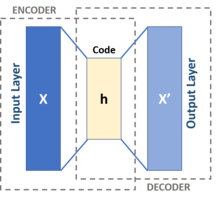
\includegraphics[width=0.4\textwidth]{images/autoencoder.png}
    \caption{Scheme of a basic autoencoder.}
    \label{fig:autoencoder}    
\end{figure}

\subsection{Development software}
MATLAB is a proprietary multi-paradigm programming language and numeric computing environment developed by MathWorks. MATLAB allows matrix manipulations, plotting of functions and data, implementation of algorithms, creation of user interfaces, and interfacing with programs written in other languages\footnote{\url{https://https://https://https://en.wikipedia.org/wiki/MATLAB}, 02/02/21}. We decided to use Matlab as Machine Learning tool because we felt more confident, while also it has an extensive documentation and it offers different advantages:
\begin{itemize}
\item Implement and test algorithms easily
\item Develop the computational codes easily
\item Debug easily
\item Use a large database of built in algorithms
\item Process still images and create simulation videos easily
\item Symbolic computation can be easily done
\item Possibility of calling external libraries
\item Perform extensive data analysis and visualization
\item Develop application with graphics user interface
\end{itemize}


\subsection{Goal of the project}
The objective of the project is to develop a compression strategy for local SURF descriptors using an autoencoder and perform a SfM reconstruction using COLMAP software with the obtained data. The matchings and the features must be saved in a .txt file. The autoencoder has to be trained with training data generated from a given dataset and has to be tested on another dataset. The final result should display a worse reconstruction due the compression of the data and the goal is to find a good setting for the autoencoder. 